\chapter{位置隐私保护技术}
\label{chap1}
本章首先介绍LBS应用模式的分类,主要分为两种:“用户提问-服务器应答”模式、“服务器提问-用户应答”模式\cite{zhanghao}。然后对位置隐私保护的系统结构进行了分类介绍,具体包括独立式结构、分布式点对点结构、中心服务器结构三个方面。之后对LBS应用中的隐私保护技术进行了介绍,最后对隐私保护技术进行对比和总结。
\section{LBS应用模式}
移动互联网与地理维度的巧妙结合,推动了LBS的快速发展。LBS应用已经渗透到了人们的衣食住行。交通部分利用LBS可以对交通拥挤路段进行分流,企业利用LBS可以更具有针对性的广告投放,民众可以利用LBS 寻找距离自己最近且性价比更高的娱乐设施。通过对LBS应用模式的总结,可以将其分为“用户提问-服务器应答”模式、“服务器提问-用户应答”模式。
\subsection{用户提问-服务器应答}
在此模式中,用户是请求的发起者。当用户需要获得LBS提供的服务时,用户通过定位设备获取到当前所在位置,然后将自己当前位置以及需求发送给服务提供商,服务器收到用户的请求后,根据用户的位置以及需求,返回给用户相应的结果。在此过程根据用户的请求方式,又可以此模式分为以下两类:
\paragraph{单次查询应用}
单次查询应用是当前应用最广泛,也是技术最成熟的模式。在此类场景中,用户发送给服务器一个当前时刻的位置信息和请求,服务器收到请求后,根据位置信息向用户提供此时此地的个性化信息,用户得到了直接的服务。如同现在的美团、大众点评就是典型的单次查询应用,可以获得距离用户此时候位置最近的影院(K近邻问题),也可以查询1公里以内最便宜的KTV(区域排序问题)。此模式中用户只提交一次或少许几次的请求查询服务,服务器得到是用户当前的静态位置。
\paragraph{连续查询查询应用}
在此模式中,用户需要持续不断的向服务器发送自己当前的位置信息。典型的应用就是现在的导航系统,用户在使用导航服务的时候,需要时时的向服务器发送自己的当前所在位置,服务器收到用户的实时位置信息后,为用户推荐正确的路线,提醒用户哪里会出现监控以及哪条路段有速度限制。此外还有如今也有不少APP需要用户实时向服务器提供当前的位置,比如微米,他能够发现此时此刻周围的好友,当你在购物的时候,如果你的好像刚好也出现在商场周围,那么APP 将会推送一条实时消息,通知你有好友也在逛街,与此同时,你的好友也会收到类似的消息。在此应用中,服务器不仅可以获得用户的静态位置,还能获得用户的运动轨迹信息。

\subsection{服务器提问-用户应答}
此模式中的角色与“用户提问-服务器应答”模式角色信息相反,此模式的服务器是请求的发起者,服务器会向用户请求一些特定的数据,用户接受到请求消息后将相应的个人数据发送给服务器。此模式中服务器可以收集到大量的用户信息,服务器可以对这些数据进行分析,挖掘出一些隐藏的有利信息。因此“服务器提问- 用户应答”模式在数据统计场景方面用的比较广泛。例如可以实时手机公交车、出租车等交通工具的位置信息,等待时间,从而预测路段的拥挤情况,及时的进行拥堵路段的车辆分流。特别的,如今电子钱包都被植入手机(支付宝、Apple Pay),商家可以利用顾客在何地消费,挖掘出潜在的商业价值,此类模式在今后的发展中应该会越来越好,伴随的应用也会随之增多。
\section{隐私保护系统结构}
在LBS中,隐私保护技术主要分为三种类别:独立式结构(Non-cooperative Architecture)、分布式点对点结构(Peer-to-Peer Architecture)、中心服务器结构(Centralized Architecture)\cite{WuYinJie}。
\subsection{独立式结构}
独立式结构\cite{ChengR}是一个典型的客户端/服务器(Client/Server,C/S)结构,主要构成部分为移动用户(客户端)与位置服务提供商(服务器),如图\ref{fig:independentConstruction_pdf}所示。独立式结构要求客户端具具有自身定位、数据存储、数据计算的能力。移动用户根据自身的隐私需求,设置合理的隐私保护方案,将自己当前位置进行匿名化处理。匿名处理完成后,用户将位置匿名结果和查询内容通过移动互联网一起发送给位置服务器;服务器在接收到请求后,根据匿名后的位置进行查询处理,并将查询结果返回给移动用户;移动用户在收到位置服务器返回的结果后,根据自己当前的真实位置选出正确的结果。


\begin{figure}[H]
\centering
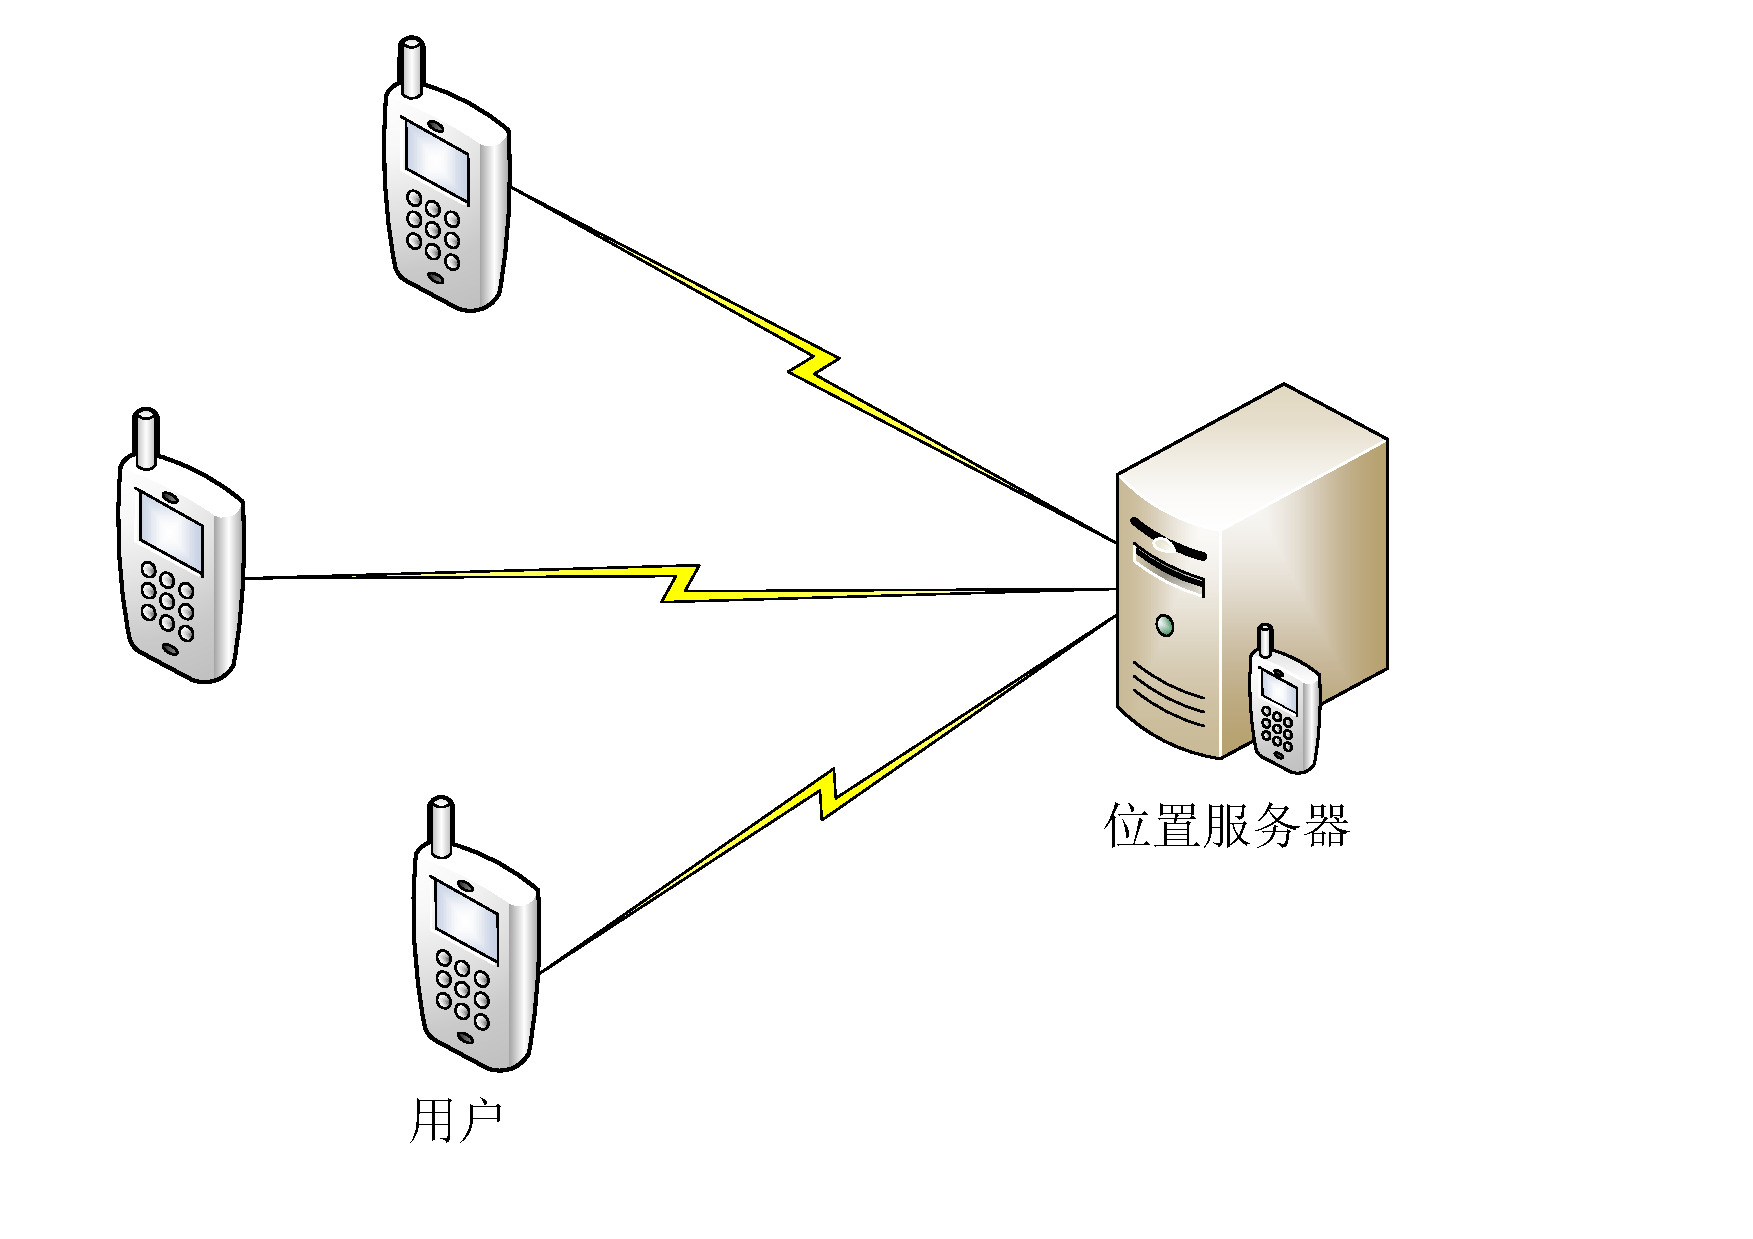
\includegraphics[width=12cm]{fig/independentConstruction.pdf}
\caption{独立式结构示意图} %\vspace*{-1.0cm}
\label{fig:independentConstruction_pdf}
\end{figure}

独立式结构主要有客户端和位置服务器两部分构成,结构简单,容易扩展。但由于客户端是独立存在的,不能达到负载均衡,因此要求客户端需要具有一定的数据计算与存储能力,而现在的可便携设备(如手机,智能手表,GPS导航仪等)的计算和存储能力都比较有限。
\subsection{分布式点对点结构}
分布式点对点结构\cite{Gruteser}同独立式结构一样,同为C/S结构,都是由移动用户和位置服务器两部分构成的。不同的是,独立式结构中的移动用户(客户端)是单独存在的个体,而分布式点对点结构中移动用户之间相互通信,构成一个群体,如图所示图\ref{fig:p2p_pdf}。 群体中的每个移动用户都是平等的,都具有一定的数据存储和计算能力的通信设备。

分布式点对点的信息请求与查询处理过程主要分为两个步骤:\Rmnum{1}.移动用户找到当前位置周围的其他用户,根据自身的隐私需求,选择合适的匿名算法,将自己位置隐匿在用户位置组当中,并将匿名后的位置发送给位置服务器。在图\ref{fig:p2p_pdf} 中,假如移动用户\ding{172}为提出查询请求的用户,用户\ding{172}的当前位置周围有用户\ding{173}、用户\ding{174}、用户\ding{175} 三个用户。用户\ding{172}选择匿名算法,将自己位置隐匿(可以将位置转为周围任何一位用户的位置,此处假设隐匿为用户\ding{174}的位置),用户\ding{174}将用户\ding{172}匿名后的位置发送给位置服务器。\Rmnum{2}.位置服务器收到用户的位置查询请求后,作出响应,并将结果返回给用户\ding{174}。 用户\ding{174} 接收到服务器端的响应后,将处理请求结果发送给用户\ding{172}。


\begin{figure}[H]
\centering
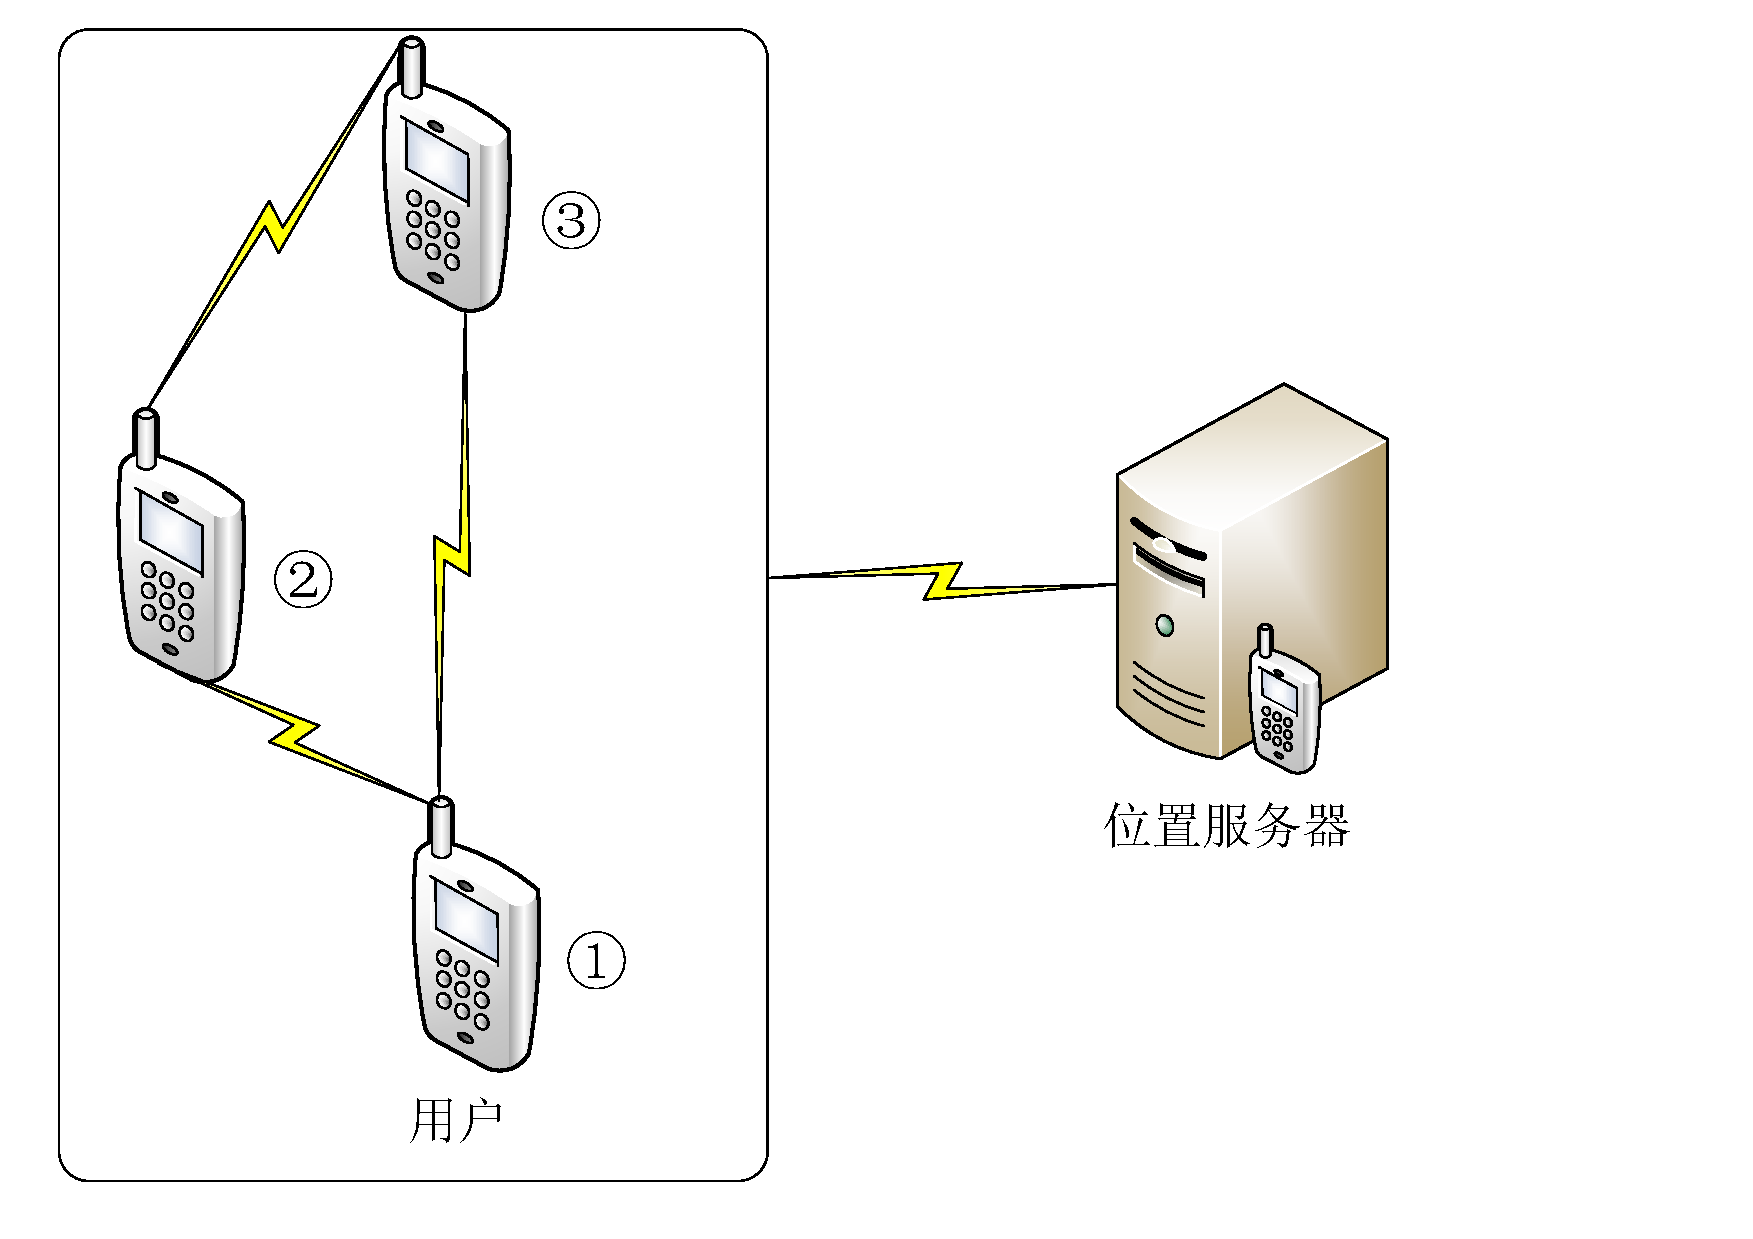
\includegraphics[width=12cm]{fig/p2p.pdf}
\caption{独立式结构示意图} %\vspace*{-1.0cm}
\label{fig:p2p_pdf}
\end{figure}

相对于独立式结构,分布式点对点结构通过分布式计算减轻了个体用户的计算和存储开销,达到了负载均衡,但是由于各个用户(客户端)之间需要互相通信,使得网络间的通信代价很高,存在通信延迟,一旦出现网络风暴,可能导致系统瘫痪,消息请求响应失败。


\subsection{中心服务器结构}
由于位置服务器通常是半可信甚至不可信的,因此中心服务器结构中移动用户与位置服务器之间不直接进行通信,而是在两者之间增加了一个可信第三方- 匿名服务器,如图\ref{fig:centralized_pdf}所示。匿名服务器主要有如下作用:1. 移动用户将当前位置的确切信息发送给匿名服务器,匿名服务器负责收集用户的位置信息,当用户位置信息发生变化后,负责更新用户的位置信息。 2. 匿名服务器在收到移动用户的确切位置信息后,根据匿名算法,将用户得精确位置信息转换为隐匿区域,并将匿名后的位置发送给位置服务器。3.位置服务器对匿名后的位置进行查询处理,将查询处理结果发送给匿名服务器,匿名服务器收到候选结果后,选择正确的响应结果发送给相应的移动用户。

\begin{figure}[H]
\centering
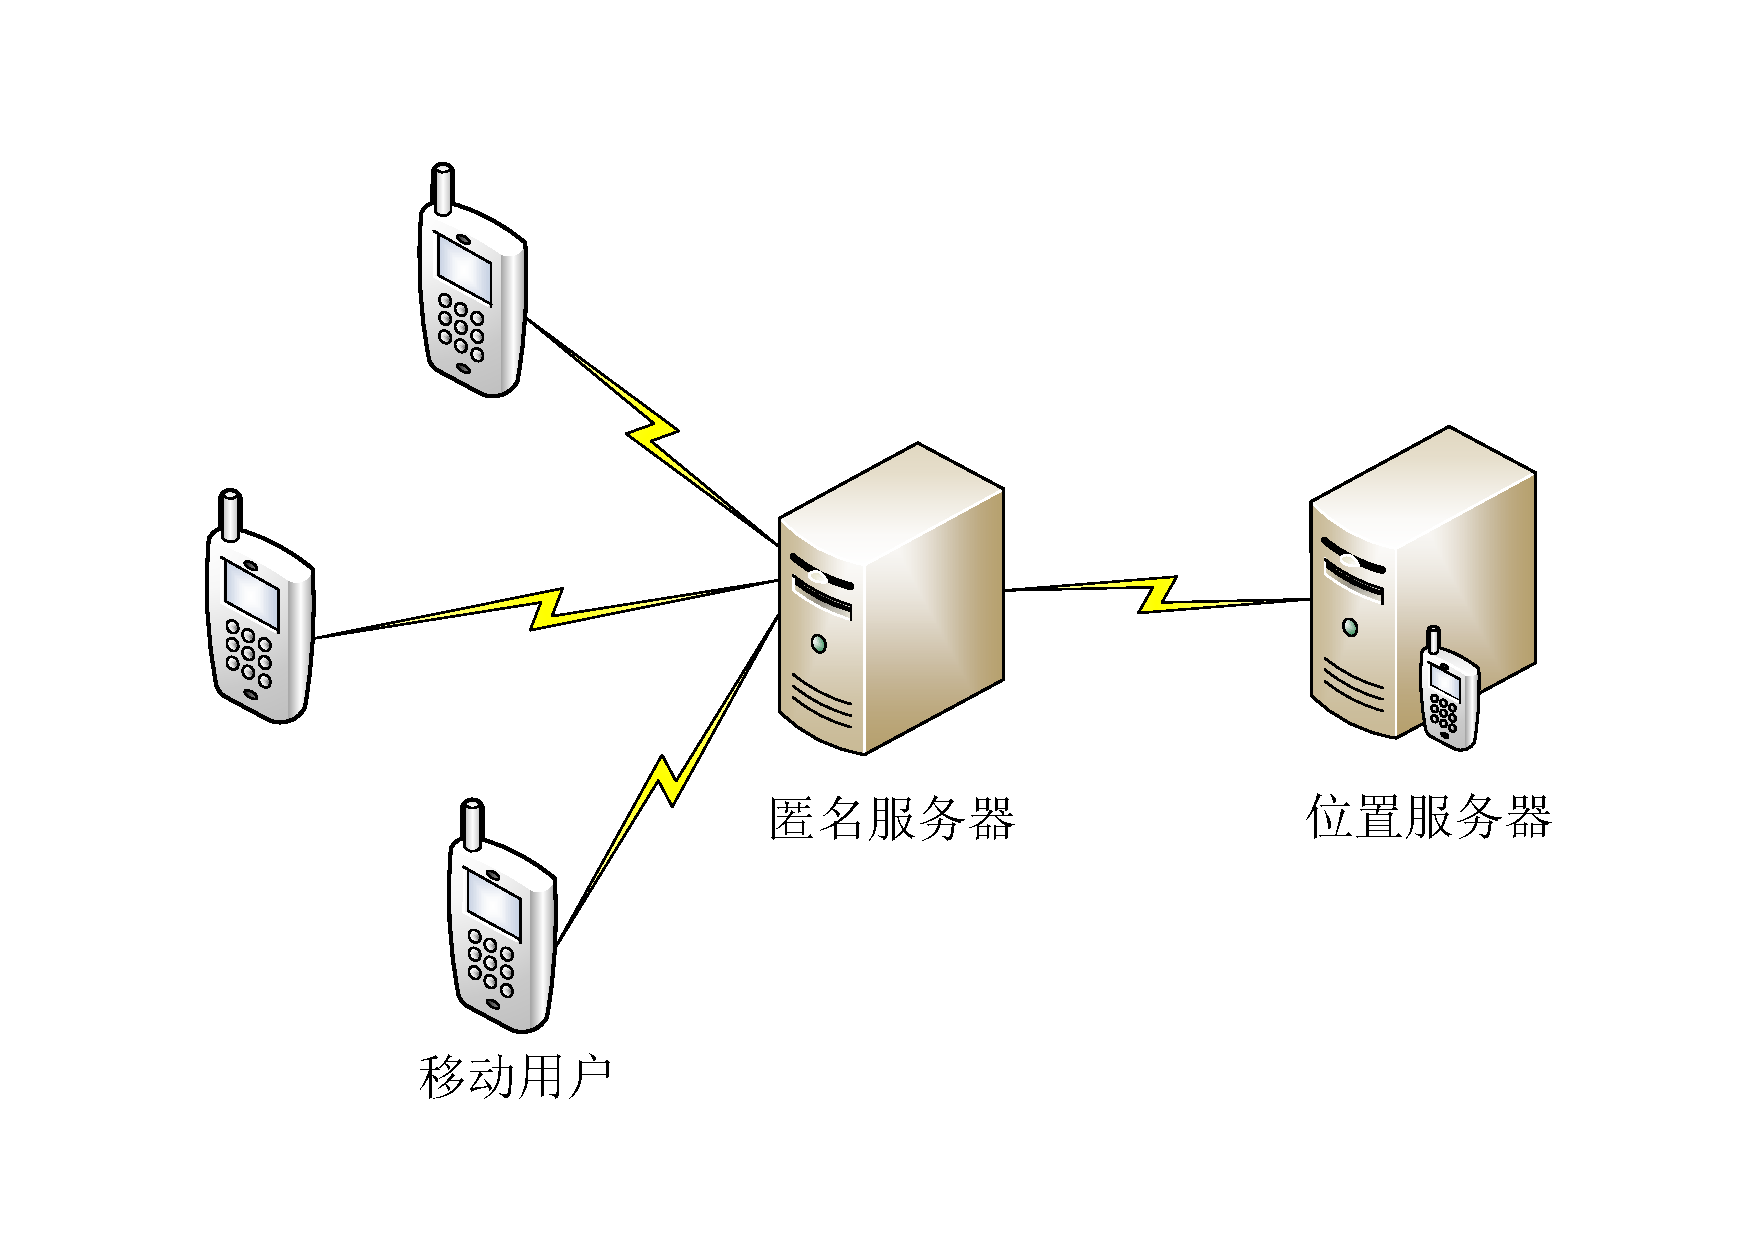
\includegraphics[width=12cm]{fig/centralized.pdf}
\caption{独立式结构示意图} %\vspace*{-1.0cm}
\label{fig:centralized_pdf}
\end{figure}

在独立式结构中位置匿名化由移动端进行处理,移动端通常是计算性能较低可便携或可穿戴设备,容易造成计算瓶颈。在中心服务器结构中,降低了移动客户端的计算和存储开销,同时还能满足用户的隐私需求。但是由于匿名服务器需要对用户的位置更新,位置的匿名进行处理,一旦操作频繁,这些请求容易成为匿名服务器的处理瓶颈。另外,匿名服务器掌握着移动用户的精确位置信息,一旦匿名服务器被敌手攻破,将会使得用户资料的泄漏。

\section{隐私保护技术}
基于位置服务的隐私保护的主要目的是用户在享受高质量的服务的同时又不会将自己的个人信息以及位置信息暴露给服务提供商。最近几年,国家大力提倡网络安全,网络空间安全也被列为教育部一级学科。与此同时,人们对LBS 应用的隐私保护问题关注度也日益高涨,国内外学者对此已有大量的研究总结\cite{group}\cite{Beresford}\cite{ChengR}。 当前LBS 应用的隐私保护研究重点集中在位置信息的隐私保护上面,我们首先给出用户发送给服务提供商的服务请求定义:
\begin{define}[:LBS服务请求]
移动用户向位置服务提供商提出查询请求R,可以抽象定义为下面的三元组:
$R=(UserID,Position,Query)$
\end{define}
其中,userID代表移动用户的唯一身份标识符,如身份证号、手机号码;而Postion可以代表一个真实的精确位置,如GPS定位中的经度和纬度,也可以代表用户所在位置的一个模糊区域。Query代表用户查询的内容,如“查询附近的影院”。

由定义2.3.1可知,可以通过对UserID进行保护处理,让服务提供商无法识别用户的ID。也可以对Position进行变换处理,让服务提供商无法通过Position获得用户的真实位置。综合这两方面,下面将详细介绍四种类型的隐私保护技术:(1) 假名技术; (2) 假位置技术; (3) 区域覆盖技术;(4) 密码学技术 。
\paragraph{基本概念}
\begin{define}[准标识符]
给定一个关系表$T$($T_1$,$T_2$,$T_3$,...,$T_n$),若表$T$能通过属性集$T^’$=\{$T_i$,$T_i+1$,...,$T_j$\} ~$\subseteq$~ \{$T_1$,$T_2$,$T_3$,...,$T_n$\} 与其他公开发布的数据进行连接,并且重新识别出实体隐私信息或部分隐私信息,则属性集$T^’$称为表$T$的准标识符,记作$QI$。
\end{define}

如表\ref{k-anony}所示的病人就诊信息表$T$,假如病情为病人的隐私信息,则隐私信息可以表示为$S$(姓名,~病情),而表$T$能通过属性{住址,~ 年龄,~性别,~ 联系方式}与其他公开发表的数据(如购物信息表)连接得到隐私信息的部分元组,则表$T$的准标识符为$QI$=\{住址,~年龄,~性别,~ 联系方式\}。
\begin{table}[hbp]
\label{k-anony}
\centering  % 表居中
\begin{tabular}{ccccc}  % {ccccc} 表示各列元素对齐方式,left-l,right-r,center-c
\hline
住址 &年龄&性别 &联系方式&病情\\ \hline  % \hline 在此行下面画一横线
上海普陀区&18 &男 &15315846561 &感冒\\         % \\ 表示重新开始一行
上海静安区 &20 &男 &15315974561 &肺炎\\        % & 表示列的分隔线
浙江嘉兴 &26 &女 &16235478951 &中耳炎\\
浙江杭州 &28 &女 &16235954123 &感冒\\ \hline
\end{tabular}
\caption{关系表T}
\end{table}

\begin{table}[hbp]
\label{k-anony-2}
\centering  % 表居中
\begin{tabular}{ccccc}  % {ccccc} 表示各列元素对齐方式,left-l,right-r,center-c
\hline
住址 &年龄&性别 &联系方式&病情\\ \hline  % \hline 在此行下面画一横线
上海*&[15-20]&男 &15315****** &感冒\\         % \\ 表示重新开始一行
上海*&[15-20]&男 &15315****** &肺炎\\        % & 表示列的分隔线
浙江*&[25-30]&女 &16235****** &中耳炎\\
浙江*&[25-30]&女 &16235****** &感冒\\ \hline
\end{tabular}
\caption{关系表$T^*$}
\end{table}

将表$T$的准表示符属性集记为$A^{QI}$,敏感属性集记为$A^S$,因此可以将表$T$简单表示为$T$($A^{QI},A^S$)。

\begin{define}[k-匿名约束]
对关系表$T$($A^{QI},A^S$),如果属性$A^{QI}$中每个元组的重复次数至少为$k$($k\geq$2),则称表$T$在属性集$A^{QI}$上满足$k-$匿名约束。
\end{define}

如表\ref{k-anony-2}所示,在属性集\{住址,年龄,性别,联系方式\}上投影得到的元组具有多重集。元组\{“上海*”,“[15-20]”,“男”,“15315******”\}的重复次数为2,元祖\{“浙江*”,“[20-25]”,“女”,“16235******”\}的重复次数也为2,因此表$T^*$在属性集\{住址,年龄,性别,联系方式\}满足2-匿名约束。
\subsection{假名技术}
假名技术属于对用户userID进行保护的一种方法,当用户向位置服务提供商发送请求的时候,采用虚假的userID代替用户的真实userID。这样位置服务提供商就无法收集userID 与位置信息的对应信息。即使存在某个攻击者获得了用户名和对应的位置信息,由于用户名是伪造的,因此不能对用户的隐私造成危害。

混淆的概念早期被应用于网络间的通讯,如今在隐私保护的应用方面也得到了各位学者的青睐。假名技术的代表就是混淆区域(Mix-Zone)技术。Mix-Zone将地图划分为两个区域:应用区域和混淆区域\cite{Mix}。 在应用区域中,用户无需做任何操作,可以正常的享受位置服务提供商所提供的服务。当用户从应用区域进入混淆区域后,用户将不能向位置服务提供商发送自己的位置信息。另外在用户离开混淆区域之前,用户将同步更新自己的身份信息,并且使用是一个之前未曾使用过的假名代替现有的名字。如图\ref{fig:mix_zone_pdf},当一个用户从混淆区域出来后,服务提供商无法将用户和当前混淆区域中的其他用户区分开来,从而实现了混淆区域中的用户的$k$-匿名保护,在攻击者看来目标用户和其他$k$-1个用户在准标识符$QI$ 上相一致。由于用户在经过不同混淆区域的时候,都会生成新的且从未使用过的假名代替当前的名字,这样使得用户信息的隐私保护程度得到了增强。
\begin{figure}[H]
\centering
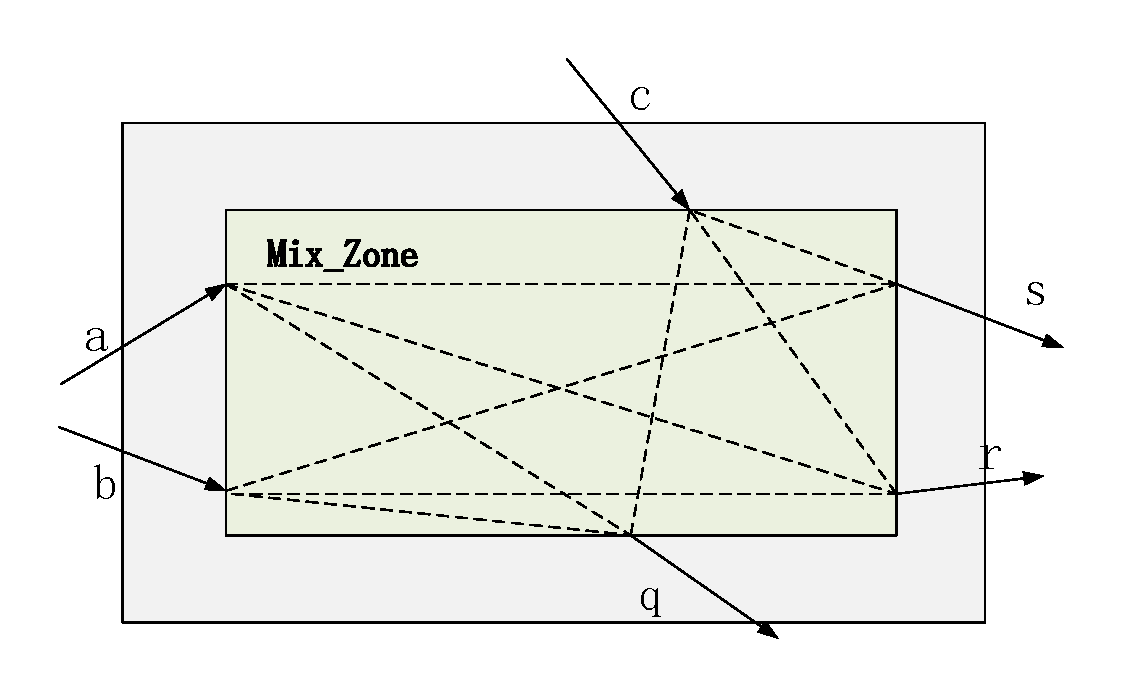
\includegraphics[width=12cm]{fig/mix_zone.pdf}
\caption{混淆区域示意图} %\vspace*{-1.0cm}
\label{fig:mix_zone_pdf}
\end{figure}
表\ref{mix}给出了拥有三个用户的混淆区域的实例,在表中,三个用户的真实身份分别为甲、乙、丙。三个用户分别在第2、5、8 个时间点进入混淆区域,且以$A$、$B$、$C$ 作为其各自的假名。之后进入混合区域2,此时每位用户又分别以新的假名$X$,$Y$,$Z$作为各自的新身份,在第7、8、12个时间点用户分别走出混淆区域。综上,我们可以得出每位用户在混淆区域内的时间分别为5、3、5。由于攻击者无法预测用户在混淆区域内停留时间的长短,当混淆区域用户人数数量较多的时候想要关联用户的身份信息难度很大。
\begin{table}[H]
\label{mix}
\centering  % 表居中
\begin{tabular}{cccccc}  % {lccc} 表示各列元素对齐方式,left-l,right-r,center-c
\hline
真实身份 &假名1&时间1 &假名2&时间2&停留时间\\ \hline  % \hline 在此行下面画一横线
甲 &A &1 &X &5 &4\\         % \\ 表示重新开始一行
乙 &B &3 &Y &6 &3\\        % & 表示列的分隔线
丙 &C &5 &Z &8 &3\\ \hline
\end{tabular}
\caption{混淆区域实例}
\end{table}

由于Mix-Zone技术限制了用户在混淆区域时任何用户都不能将自己的位置发送给位置服务提供商,当用户进行持续位置服务请求的时候(例如导航),混淆区域技术就不能满足这方面需求,因为用户会有一段时间进入“盲区”。另外混淆区域的大小,以及混淆区域内用户的数量,也会对隐私保护的质量带来一定的影响。

\subsection{假位置技术}
在发布假位置技术中,用户将自己当前的真实位置以及生成的假位置发送给位服务提供商。提供商根据每个位置信息作出响应,并将响应消息发送给用户,用户收到反馈信息后,仅从中抽取真实信息。图\ref{fig:Dummy_pdf}描述了假位置的LBS服务过程,其步骤主要如下:	

\ding{172}~用户通过定位设备获得位置信息$P_1$。

\ding{173}~生成假位置$D_1$和假位置$D_2$。

\ding{174}~用户将请求消息S($P_1$,$D_1$,$D_2$)发送给服务提供商。

\ding{175}~服务提供商对所有位置信息进行查询,并将响应消息$R$发送给用户。

\ding{176}~用户从$R$中选出正确的消息T。
\begin{figure}[H]
\centering
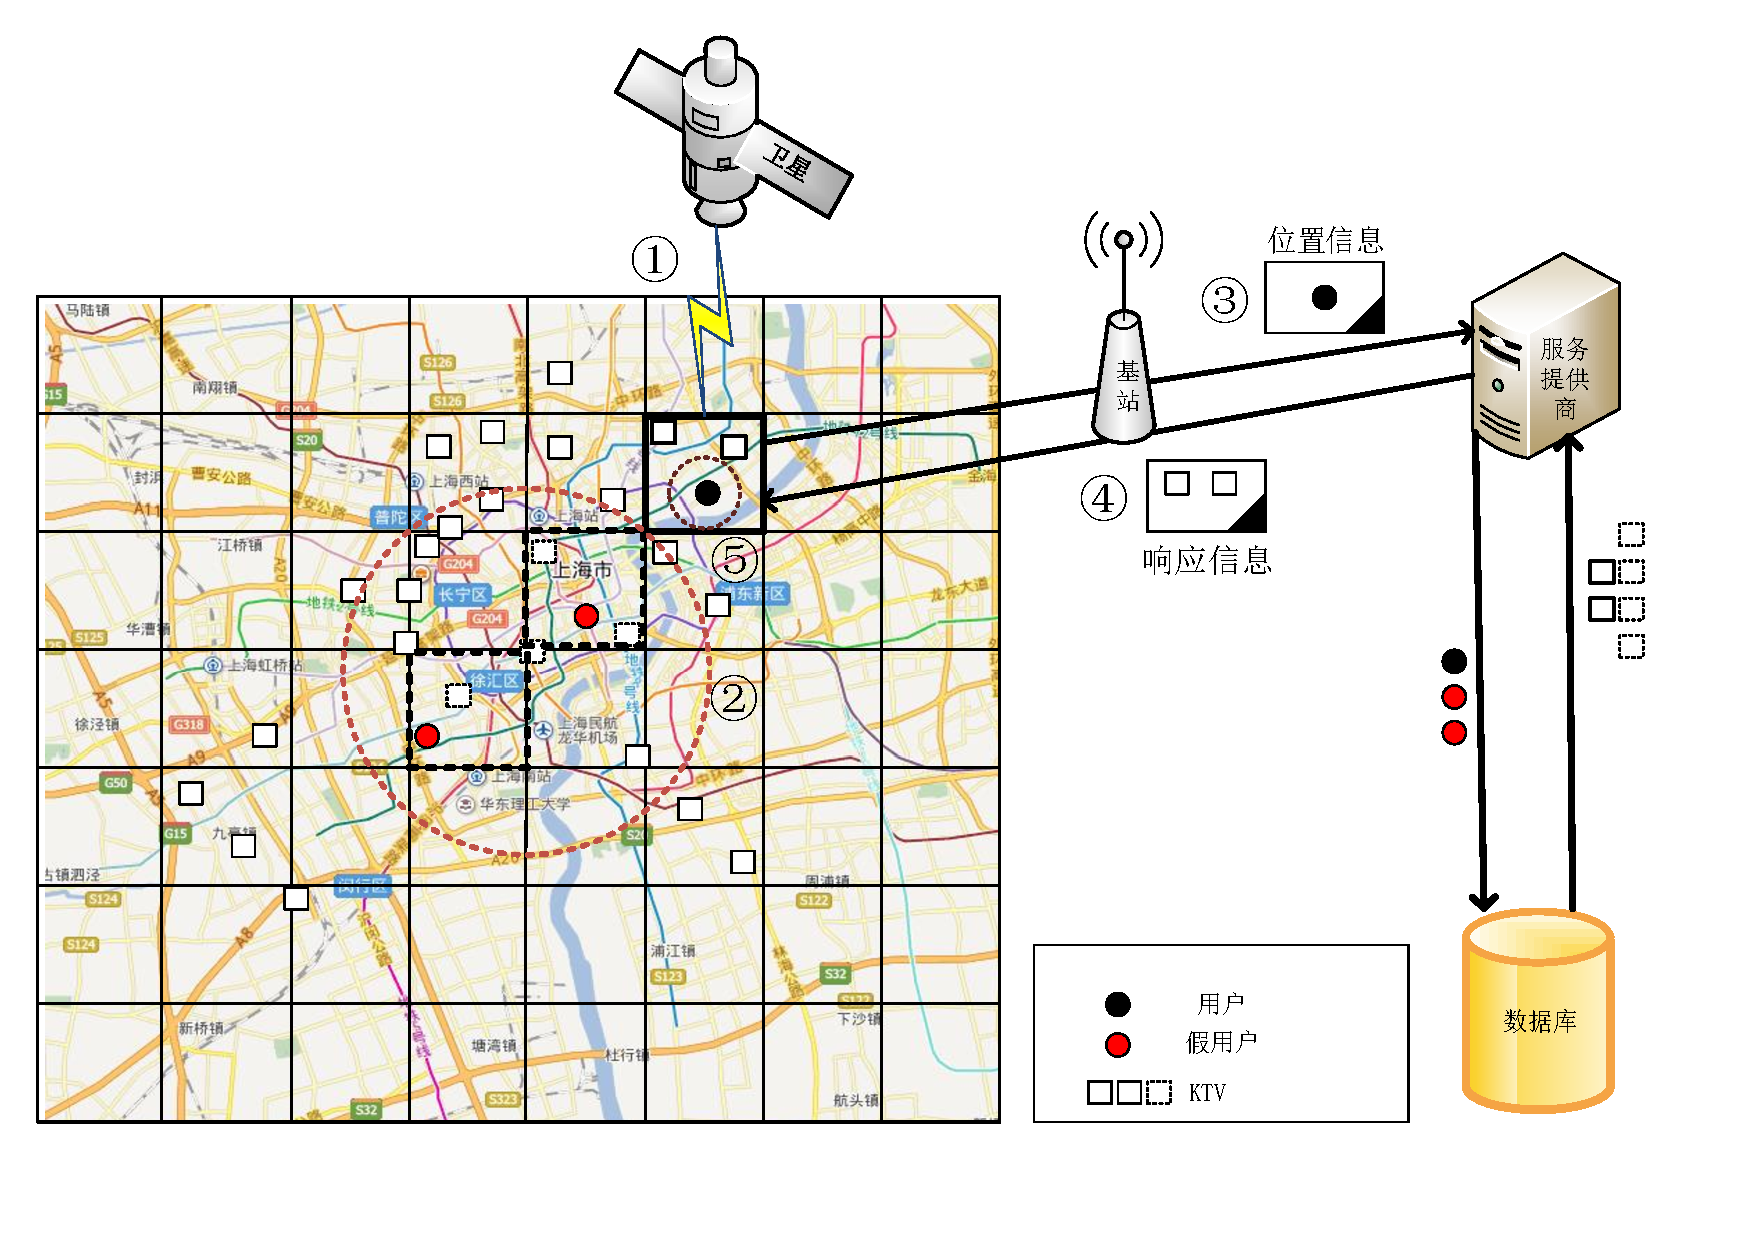
\includegraphics[width=12cm]{fig/Dummy.pdf}
\caption{假位置通信图} %\vspace*{-1.0cm}
\label{fig:Dummy_pdf}
\end{figure}
在这当中核心部分就是如何生成假位置集,通常情况下考虑位置匿名性的程度从两方面考虑:\\
\textbf {普遍性} 普遍性是指分布在每个区域中,如图\ref{fig:subfig:a}。当所有用户当住在同一个区域中,那服务器很容易列举出个一些户,而当用户分布各个区域后,服务器就很难列举出。因此普遍性可以提高整个区域内的用户位置匿名。\\
\textbf {密集性} 密集性是指大量用户处在同一个区域,如图\ref{fig:subfig:b}。这思想主要来源于K匿名,用户在某个区域中发送位置信息给服务器,由于此区域存在大量的用户,服务器很难指定出某个用户,因此密集性提高了某个区域用户位置的匿名。


由于普遍性考虑的是整个区域内用户的位置隐私,而密集型考虑的是局部用户的位置隐私,因此本节将主要围绕普遍性进行叙说。

在\cite{Dummies}种,Hidetoshi Kido提出的Dummys的算法中,用户每次讲将自己的真实位置和随机生成的假位置发送给服务提供商,这其中并没有考虑到重复单次查询下的聚合攻击。比如用户通过手机向大众点评请求相关服务,第一次用户查询当前位置$P_1$周围的影院,用户将真实位置$P_1$ 以及两个假位置$D_2$,$D_3$发送给服务器。第二次用户查询当前位置$P_1$ 周围的KTV,同样将$P_1$以及假位置$D_3$,$D_4$发送给服务器。由于用户每次发送的位置集合中必有一个是用户的真实位置,因此服务器可以通过对两次请求进行求交集,即求($P_1$,$D_1$,$D_2$)~$\bigcap$~($P_1$,$D_3$,$D_4$),结果显然为$P_1$,即为用户的真实位置,因此用户的位置隐私得不到保护。

\begin{figure}
 \centering
 \subfigure[普遍性]
 {
    \label{fig:subfig:a} %% label for first subfigure
     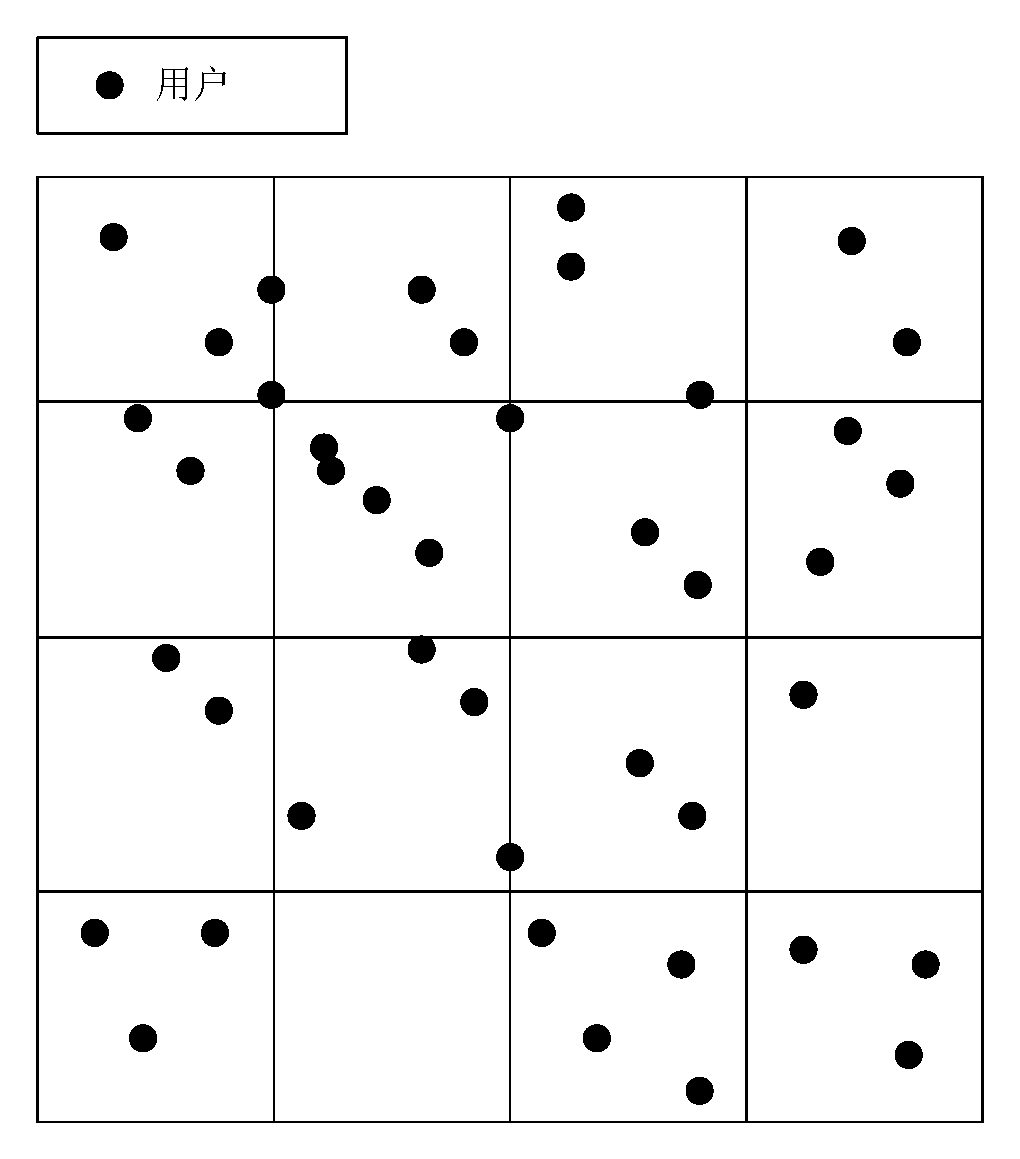
\includegraphics[width=2.0in]{fig/ubiquity.pdf}
 }
 \hspace{1in}
 \subfigure[密集性]
 {
   \label{fig:subfig:b} %% label for second subfigure
   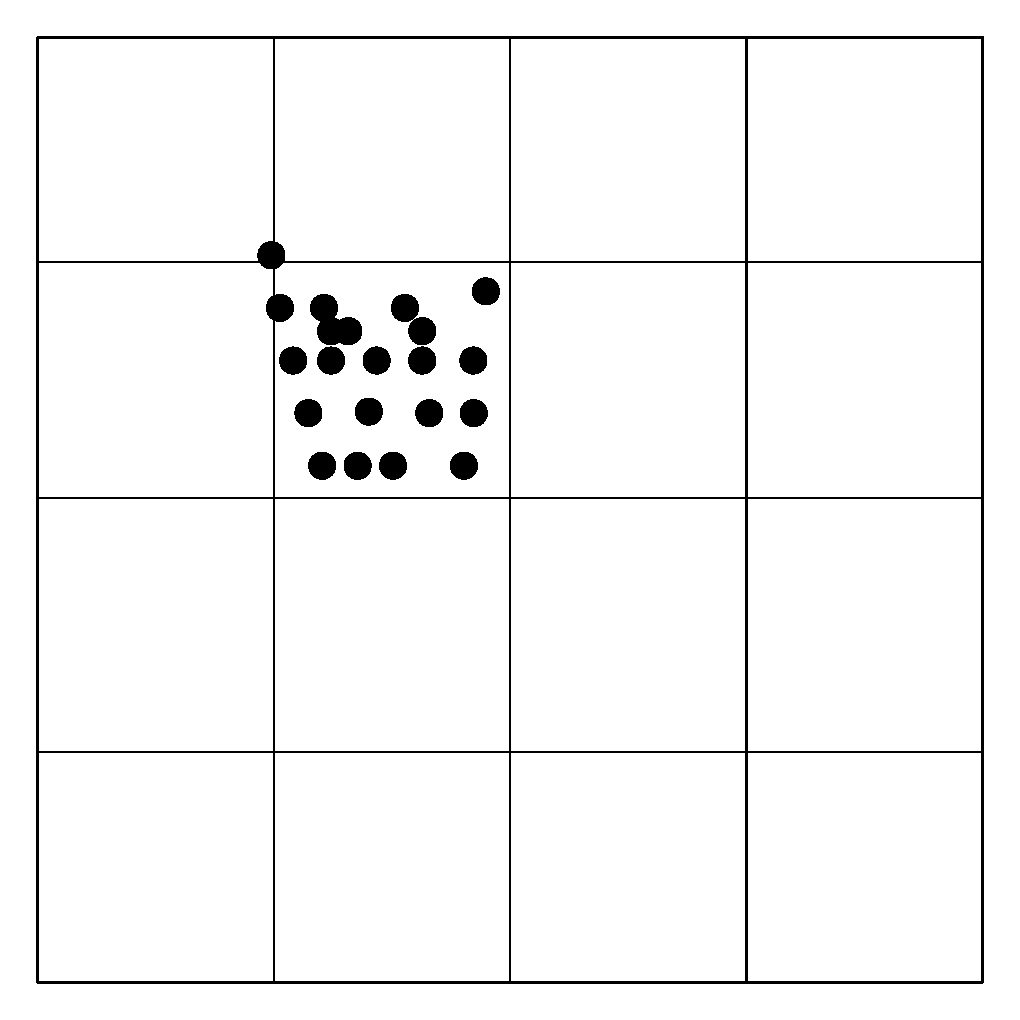
\includegraphics[width=2.0in]{fig/congestion.pdf}
 }
 \caption{普遍性和密集性示意图} \label{fig:subfig} %% label for entire figure
\end{figure}
同样,如果用户每次都使用相同的假位置,而不是进行随机的选择,此方法可以避免用户在相同位置下的聚合攻击,但一旦用户的位置发生变化,那么无法抵抗连续查询下的聚合攻击。例如用户在位置$P_1$时向服务器提出查询,此时将位置集合($P_1$,$D_1$,$D_2$)发送给服务器。当用户的位置发生变化,用户在位置P2时,向服务器提出查询,并将位置集合($P_2$,$D_1$,$D_2$)发送给服务器。服务器通过求后一个状态和前一个状态集合的差集,即($P_2$,$D_1$,$D_2$)-($P_1$,$D_1$,$D_2$),结果为$P_2$,因此服务器便能得出用户当前时空下的位置信息。

针对上述的情况,本节将在假位置的基础上提出一种新的位置匿名算法,此算法即能抵抗用户静止状态下的连续查询聚合攻击,又能抵抗用户在非静止状态下的连续查询聚合攻击。算法主要由一下几部分组成:
基于上述描述过程,伪代码如代码\ref{alg:Dummy}所示:

\ding{172}~假位置生成,用户随机生成一定数量的假位置集合$D$。

\ding{173}~位置获取,用户通过定位设备获取自己当前位置$P_c$。

\ding{174}~状态获取,获取用户的上一个位置状态信息$P$。

\ding{175}~状态判断,判断当前位置是否和当前位置存在偏差,若偏差达到一定的阈值$m$,则转至\ding{172},获取新的假位置集合$D_N$。

\ding{176}~请求发送,将真实位置和假位置组成的位置集合发送至服务器。

\ding{177}~响应反馈,服务器将响应信息返回至用户。

\ding{178}~信息筛选,用户从响应消息中筛选出正确的信息。\\
\begin{algorithm}[!htb]
\small
\renewcommand{\algorithmicrequire}{\textbf{Input:}}
\renewcommand{\algorithmicensure}{\textbf{Output:}}
\caption{生成假位置集合}
\label{alg:Dummy}
\begin{algorithmic}[1]
    \REQUIRE 用户上一个查询位置$P$,预先设定假位置集合$D$={$D_1$,$D_2$,$D_3$,...,$D_k$},区域$R$,阈值$m$
    \ENSURE 位置集合$D_N$=($D_{N_1}$,$D_{N_2}$,$D_{N_3}$,...,$D_{N_K}$)
    \STATE $D_{N_1} \gets Random(0,R)$
    \FOR {$i \gets $ 2 to $K$}
        \STATE $D_{N_i} \gets $ Random($D_{N_i-1}-m,D_{N_i-1}+m$)
        \IF{$D_{N_i}~~equals~~D_{N_i-1}$}
            \STATE $D_{N_i} \gets Random(D_{N_i},D_{N_i}+m)$
        \ENDIF
    \ENDFOR
    \STATE $P_c \gets$ 用户获取当前实时位置
    \IF{$P_c~-~P$ < $m$}
        \STATE $M \gets$ $(D_1,D_2,D_3,...,D_k)$
    \ELSE
        \STATE $M \gets $ $(D_{N_1},D_{N_2},D_{N_3},...,D_{N_k})$
    \ENDIF
\end{algorithmic}
\end{algorithm}

\subsection{区域覆盖技术}
区域覆盖技术是位置隐私保护中常见的方法之一\cite{Mokbel}\cite{xu2010privacy}\cite{xu2009feeling}。 该方法的主要思想是将用户精准的位置信息用一个模糊的区域代替,用户在发送请求的时,并不将自己的位置发送给服务器,而是所在区域的某一模糊区域发送给服务器。区域覆盖技术将用户隐藏在一定大小的区域内,使得他人无法获得目标的准确位置。覆盖区域根据实际情况进行选择,一般有圆形覆盖区域和矩形覆盖区域。圆形覆盖区域看起来最为直观和自然\cite{ardagna2007location}\cite{kalnis2007preventing},然而将地图划分为圆形区域会产生大量的重叠,而且在计算和表示等方面都没有矩形区域方便。因此目前最为普遍的区域划分法为矩形区域划分,此划分法将地图划分为若干个互补相交的矩形区域,实现对区域更好的粒度控制。另外文献\cite{wang2009privacy}\cite{hossain2011h}给出了一些不规则的区域划分,例如结合道路的形状将用户的位置以星形区域进行覆盖。

在其中基于$k$-匿名的保护方式最为广泛\cite{Bamba}\cite{Mokbel}\cite{wang2010device}\cite{pan2012protecting}, 很显然,如果一个区域中包含$k$个移动用户,那么当攻击者得到用户所在的区域时,攻击者无法区分出当前发出请求的为哪一个用户,从而这个区域实现了对移动用户位置隐私的$k$-匿名保护。如图\ref{fig:cloaking_pdf},用户A使用模糊区域(虚线区域)代替自己当前的精确位置,模糊区域中包含其他两位用户,因此模糊区域实现了$k$=3的匿名保护。$k$-匿名亦存在若干的缺点\cite{juncheng2014potential}。为解决这些缺点,出现了$k$-匿名的加强版$l-diversity$\cite{machanavajjhala2007diversity},$t-closeness$\cite{li2007t} 等技术,使得攻击者更难得到用户的信息。 一般来说,构造的模糊区域越大,模糊区域中包含的用户就会越多,$k$- 匿名保护中的$k$ 值也就越大,从而隐私保护程度就越高。但这样会给服务器带来更多的计算和通信开销,造成服务器响应延迟,导致服务器服务质量下降。因此区域覆盖技术实际上是通过消耗服务质量来提高隐私保护程度。如何在服务质量和隐私保护程度之间寻求一个平衡点,一直是国内外学者的研究热点。
\begin{figure}[H]
\centering
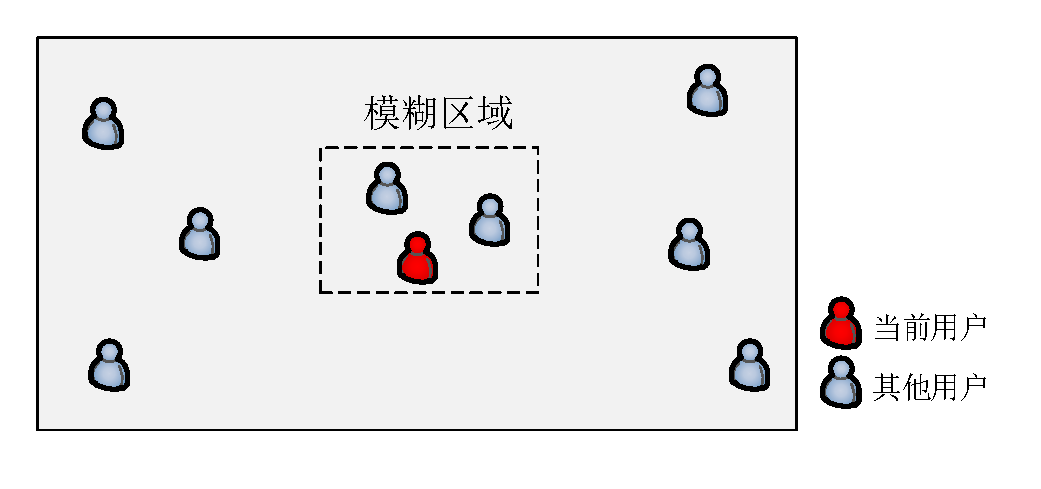
\includegraphics[width=12cm]{fig/cloaking.pdf}
\caption{空间覆盖实例} %\vspace*{-1.0cm}
\label{fig:cloaking_pdf}
\end{figure}

SSS每个用户对$k$-匿名中的$k$要求可能有所不同,文献\cite{Mokbel}中,Casper将区域划分为正方形网格,以金字塔的结构对区域进行管理,尽可能的生成用户要求的最小覆盖区域。Casper假设存在一个可信第三方机构——中心代理,中心代理负责将区域划分为$L$+1层(即金字塔的层数为$L$+1),每一层都是对区域的一种划分方式,自上而下划分粒度越来越细。在第一层,只有一个正方形方格,代表将整个区域作为一块方格,第一层粒度最粗(相当于没有划分)。之后每一层的方格数都是由上一层的方格分裂为4个小方格组成的,例如第二层为第一层的1个方格分裂出来的4个方格,第三层为第二层的4个方格分裂出来的16 个方格,图\ref{fig:GoldTower_pdf}给出了前三层的划分结构。当可信代理收到用户的请求后,采用自底向上的请求方式,先查看$L$层中用户位置所在的方格,然后查看所在方格中的其他用户数量$USERS_L$ 是否满足用户提出$k$- 匿名保护中$k$的值,如果满足,则返回$L$层的覆盖区域给用户,否则在同一层查看水平相邻的单元格中用户数量$USERS_{RL}$和竖直相邻单元格中用户数量$USERS_{CL}$, 计算$max$\{$USERS_L$+$USERS_{RL}$,$USERS_L$+$USERS_{CL}$\},若得到的值满足用户对$k$的要求则返回两个单元格,否则在上一层$L$-1层中进行查找。
\begin{figure}[H]
\centering
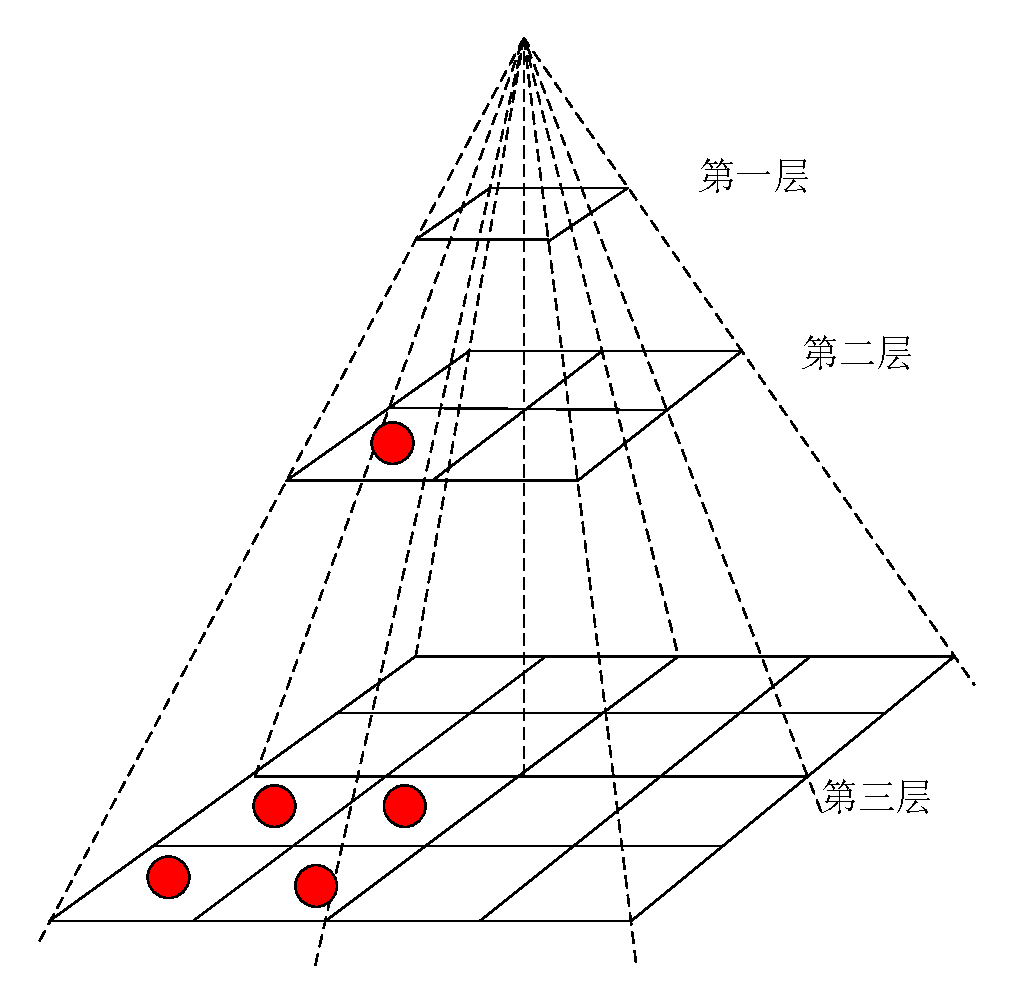
\includegraphics[width=8cm]{fig/GoldTower.pdf}
\caption{金字塔划分实例} %\vspace*{-1.0cm}
\label{fig:GoldTower_pdf}
\end{figure}
\subsection{基于密码学的隐私保护技术}
基于密码学的隐私保护技术通常是依靠密码学中存在的一些计算困难问题构造出数据隐私保护的方法。相比于之前介绍的位置隐私保护技术,基于密码学的技术对位置隐私保护更加安全,从理论上杜绝了攻击者的威胁。其中典型的代表有安全多方计算(Secure Multi-Party Computation, SMPC)和隐私消息恢复(Private Information Retrial,PIR)技术的使用。

SMPC 最早由华人计算机科学家姚期智于1982 年提出\cite{}。 具体来讲就是有$n$个参与者$P_1$,$P_2$,$P_3$,...,$P_n$希望共同计算某个约定的函数$f$($x_1$,$x_2$,$x_3$,...,$x_n$)~=~($y_1$,$y_2$,$y_3$,\\ ...,$y_n$),其中$x_1$,$x_2$,$x_3$,...,$x_n$ 分别为参与者$P_i$($i ~\epsilon ~[1,n]$) 的保密输入信息,$y_1$,$y_2$,$y_3$,...,$y_n$分别为参与者$P_i$的输出。这里的安全性是指即使在某些参与者有欺骗行为的情况下,仍然能够保证结果的正确性,即在计算结束后每个参与者$P_i$都能够得到正确的输出$y_i$,并且除了知道自身的输出$y_i$外,不能得到其他参与者的任何信息。安全多方计算协议目前已有大量的研究\cite{},其中文献\cite{126}介绍了安全多方计算的模型:半可信模型和恶意模型。文献\cite{126,128}介绍了安全多方计算所面临的一些挑战。文献\cite{129,130}介绍了如何利用安全多方协议进行隐私保护方案的设计。

PIR技术使得服务器在对用户信息一无所知的情况下还能对用户的请求提供正常的服务。文献\cite{89}基于二次剩余的假设\cite{97}构建了一个寻找最近邻兴趣点(POI)的方法,通过随机选取两个大素数$p$和$q$,数$N$=$p\star q$,判断一个数是否为模$N$的二次剩余是一个数学难题。图描述了该PIR




\section{本章小结}
\paragraph{兴趣点和兴趣区域挖掘}

兴趣点和兴趣区域通常作为推荐元素向用户推荐,在不同的挖掘任务中,根据推荐的目标不同采用的方法也不同,聚类是发现轨迹数据特征的最常用方法之一,而对于时空特性明显的地理位置数据,聚类算法的设计、度量方法的选择、数据查询结构等均是该部分的主要研究内容。本文以打车推荐为目的,重点讨论采用基于密度的聚类方法对候选扬招点和热门目的地的挖掘方法。


